\subsubsection{Goal 3: Consequences of independence-based planning}

We next examined the practical consequence of following an independence-based sample size planning strategy, as in Barnhart et al.~\cite{barnhart_sample_2025}, when the underlying true endpoint dependence is stronger than assumed at the design stage. Specifically, for each scenario, the total sample size $N$ was first determined under $\rho=0$ to achieve 85\% nominal power for WR. Then, the obtained total sample size $N$ was held fixed as the latent correlation $\rho$ increased from 0 to 0.8, and the corresponding empirical power was estimated. Figure~\ref{fig:wr_emp_power_by_scenario} displays the resulting empirical power of WR across $\rho$, thereby showing directly how achieved power changes when independence-based planning is applied to correlated hierarchical endpoints.

The practical consequence of independence-based planning was strongly scenario-dependent. In S1, the design planned under independence became mildly conservative at stronger dependence, with empirical WR power increasing from 85.1\% at $\rho=0$ to 90.6\% at $\rho=0.8$. In contrast, in S2--S4, the same planning strategy became increasingly anti-conservative: empirical WR power declined from 85.8\% to 73.7\% in S2, from 84.0\% to 70.6\% in S3, and from 85.6\% to 70.3\% in S4 as $\rho$ increased from 0 to 0.8. Thus, ignoring dependence led to mild overpowering in the S1 setting, but substantial underpowering in the remaining settings.

\begin{figure}[ht!]
    \centering
    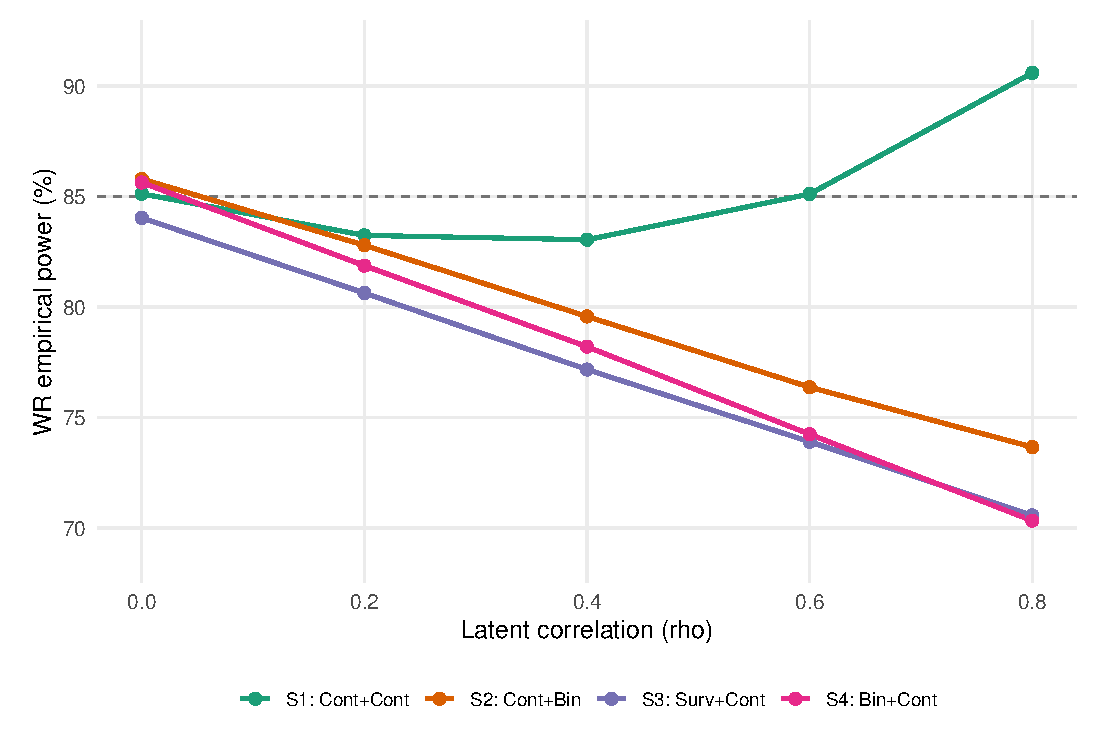
\includegraphics[width=0.6\linewidth]{Simulation Examples/Plot.WR.EmpiricalPower.ByScenario.pdf}
    \caption{Empirical power of WR across latent correlation levels $\rho$ under independence-based planning. For each scenario, the total sample size $N$ was determined under $\rho=0$ and then held fixed as $\rho$ increased.}
    \label{fig:wr_emp_power_by_scenario}
\end{figure}

These results also help explain why our conclusions differ from those of Barnhart et al.~\cite{barnhart_sample_2025}, who reported only a modest impact of dependence on power in the settings they examined. Our findings do not contradict theirs; rather, they suggest that the practical importance of dependence is highly scenario-specific. In some settings, dependence may remain relatively unimportant because the lower-priority endpoint contributes little additional tie-breaking information or because dependence affects conditional win and loss probabilities in a broadly symmetric way. In other settings, however, dependence can materially alter power when the lower-priority endpoint remains influential and dependence changes conditional win and loss information asymmetrically.

To ensure that this finding was not an artifact of the equal-variance or tie-only variance approximations used in earlier planning formulas, we conducted an additional sensitivity analysis in Appendix~\ref{app:equal_variance_sensitivity}. In that analysis, the marginal endpoint distributions, marginal treatment effects, and observed WR/NB estimates were held fixed, and only the variance coefficient used in the power formula was changed: the FORSS variance under $H_A$, the corresponding variance under $H_0$, or the Yu--Ganju tie-only approximation. Across scenarios, replacing the $H_A$ variance by the $H_0$ variance changed the calculated power only modestly relative to the much larger empirical power changes induced by increasing dependence. Thus, the underpowering observed in S2--S4 is not explained by the equal-variance approximation; rather, it reflects the way dependence changes the overall win/loss contrast itself.

In practice, the internal dependence structure of a planned HE is typically not known well enough at the design stage to determine in advance which of these situations applies. We therefore recommend using FORSS with dependence sensitivity analysis or pilot-data-based calibration described in Section~\ref{subsec:dependence-forss}, rather than relying on an independence-based sample size calculation alone. Specifically, Strategy~1 provides a practical approach when only a plausible range of dependence values can be elicited, whereas Strategy~2 can be used when pilot or historical data are available to calibrate the working dependence structure to observed concordance summaries. These strategies help reduce the risk of materially underpowered designs when dependence is more consequential than assumed under independence.
